\documentclass[10pt]{article}
\usepackage[T1]{fontenc}
\usepackage{lmodern}
\usepackage[margin=24mm]{geometry}
\usepackage{amsmath,amssymb,booktabs,tabularx,graphicx}
\usepackage{microtype}
\usepackage[colorlinks=true,linkcolor=blue,citecolor=blue,urlcolor=blue]{hyperref}
\setlength{\parskip}{3pt}
\newcommand{\BA}{\mathrm{BA}}
\newcommand{\R}{\mathbb{R}}
\newcommand{\pp}{\,\mathrm{pp}}
\newcommand{\repo}{https://github.com/20171806011/Temporal-Attention-Neuron}
\hypersetup{pdftitle={Event Replay and Evicted-Key Competition in a Native-Spike Key-Value Memory},pdfauthor={Li Zexu}}

\title{Event Replay and Evicted-Key Competition\\in a Native-Spike Key--Value Memory}
\author{Li Zexu}
\date{11 November 2026 \textbullet{} Unreviewed research manuscript}

\begin{document}
\maketitle

\begin{abstract}
In a recurrent spiking circuit with explicit key--value slots, retaining the correct value does not ensure that the circuit can express it. Earlier writes can change the recurrent state from which a later cue is read. We study this distinction in a 180-parameter dendritic population with two FIFO slots and a learned bilinear matcher. Fixed-weight substitutions implicated the native recurrent state more strongly than the stored values in one interference assay. A causal policy then reconstructed the native state by replaying visible events, omitting writes whose records were no longer retained. On 12 new training blocks, this policy improved recent-record balanced accuracy by 5.273 percentage points (97.5\% block-bootstrap interval [3.418, 7.161]) relative to the original circuit. A separate 12-block confirmation tested a veto that compares the query with evicted keys. On near-neighbor three-write histories, it improved evicted-target balanced accuracy relative to old replay by 0.781 points [0.130, 1.563], restoring the original circuit's 59.115\%. The recent-record difference was zero in all 12 blocks, retaining old replay's 96.094\%. The veto removed 16,512 replay sample steps across the final evaluation. Complete isolated calls showed geometry-dependent latency differences. These findings identify a selective repair of a specific interference pathway on short synthetic sequences.
\end{abstract}

\section{Introduction}
Key--value memory separates the address used to find a record from the value it contributes to a response \cite{miller2016}. Attention provides a general mechanism for forming a weighted combination of stored values \cite{vaswani2017}. In a spiking recurrent circuit, that combination enters a dynamical system whose earlier states can persist until the read. Address quality, value quality, and the state of the receiving circuit can therefore constrain performance separately. A retrieved value may be appropriate while the state from which the circuit must act still reflects earlier interference.

We ask three questions. First, does learned key matching affect the native spike-count answer, and where does interference reside after the FIFO has evicted a record? Second, can the circuit improve reads of retained records by reconstructing its state from causal, visible events? Third, when an evicted key competes with a retained key, can a veto suppress harmful reconstruction while preserving the benefit for retained records?

This work extends the Temporal Attention Neuron (TAN) research programme and its native-spike population studies \cite{tanrepo,populations}. The final model uses a dendritic population and explicit two-slot memory. The repository's original TAN cell instead uses temporal self-attention and a surprise gate. We distinguish those mechanisms throughout. The main evidence comes from two separately frozen, independently audited confirmation cohorts. Earlier fitted-weight interventions and engineering trials motivated the policies and supply mechanism checks.

\section{Circuit, memory, and task}
\subsection{Native dynamics and learning}
The native population has 12 graded branches, six spiking hidden somata, and two spiking outputs. Let $x_t\in\R^6$ be the input, $p_{t-1}$ the previous six hidden spikes, and $d,v,o$ the branch, soma, and output states. The forward dynamics are
\begin{align}
 z_t &= x_t W_{\rm in}+p_{t-1}W_{\rm rec}, \\
 d_t &= 0.95d_{t-1}+0.25(z_t+b_d+a_t), \\
 \tilde v_t &= 0.85v_{t-1}+0.5P[\max(d_t,0)]+b_v, \\
 \tilde o_t &= 0.85o_{t-1}+p_{t-1}W_{\rm out}+b_o.
\end{align}
$P$ sums adjacent branch pairs. Each hidden and output spike is the indicator that its candidate exceeds $0.5$. The corresponding post-spike state is multiplied by one minus the spike. The native state used for reconstruction is $(d,v,o,p)$ with 26 scalars. The system has 176 native parameters and four matcher parameters. Forward evaluation uses hard spikes and resets. The training implementation substitutes a surrogate derivative in the backward pass, following the broad approach used for hard-spiking networks \cite{zenke2018}.

Each episode has 36 steps. The two output counts $C_0,C_1$ sum spikes at $t=28,\ldots,35$. Prediction is the larger count. Ties count as incorrect and reduce coverage, the fraction of episodes with unequal counts. Balanced accuracy (BA) is the mean of the two class recalls. Training uses binary cross-entropy with logit $0.5(C_1-C_0)$ and penalty $10^{-4}\operatorname{mean}(\theta^2)$. Each fit starts from a fresh initialization, with the four matcher parameters set to zero. Training uses 128 nominal two-record episodes, 600 full-batch Adam updates, learning rate $0.0025$, $\beta=(0.9,0.999)$, $\epsilon=10^{-8}$, global gradient-norm clipping at 1, and parameter clipping to $[-2,2]$. The replay and veto policies are applied after fitting.

\subsection{Two-slot addressing and held-out histories}
At each write, the FIFO inserts the visible two-dimensional key and a 12-dimensional value $\tanh(z_t)$ and shifts the most recent record into the older slot. Value states decay with factor $0.97$ at every step. At a read, a visible query $q_t$ is mapped by a learned $2\times2$ matrix $M$. The two pre-write slot keys $k_i$ are scored by $4k_i^{\mathsf T}(q_tM)^{\mathsf T}$. A softmax over these scores weights the two pre-write values. The resulting value mixture is multiplied by $2(1-g_{\rm write})\min(1,\|q_t\|_2)$ to obtain the dendritic injection $a_t$.

The held-out task varies four potential write positions, binary contents, a selected query position, a common random key rotation, a random write order, and bounded query noise. A query is a noisy 90-degree rotation of its target key. The orthogonal geometry uses relative angles $(0,90,180,270)$ degrees. The near-neighbor geometry uses $(0,40,180,230)$ degrees. The four histories keep all writes, keep the first early write and the last two, keep the second early write and the last two, or keep only the last two. A query to a written but discarded record is labeled \emph{evicted}. A query to an omitted write is labeled \emph{missing}. A query to either last position is labeled \emph{recent}. The task generator uses a matched factorial design in each block. For missing targets, opposite labels can correspond to the same visible sequence. This gives a direct control on accuracy attributable to unavailable content.

\begin{table}[htbp]
\centering
\caption{Frozen held-out schedules. The read cue lasts three steps, and native output counting starts at step 28. Write positions omitted by a history provide no write input.}
\label{tab:schedules}
\begin{tabular}{lccc}
\toprule
Schedule & Potential writes & Nonwrite drives & First read \\
\midrule
A & 0, 3, 6, 11 & 2, 8 & 22 \\
B & 1, 4, 7, 13 & 0, 10 & 24 \\
C & 0, 2, 5, 10 & 1, 8 & 20 \\
D & 2, 5, 8, 12 & 3, 6 & 23 \\
\bottomrule
\end{tabular}
\end{table}

\section{Interventions and evaluation}
\subsection{Causal replay and the evicted-key veto}
The original circuit uses the native state already present when the cue arrives. Old replay checks the first rising read edge, whether a write has evicted a record, and whether the maximum valid cosine between the mapped query and a live key is at least $1/\sqrt{2}$. On a trigger, replay builds a length-$t$ input prefix using the logged times and vectors of the two retained writes and all visible nonzero nonwrite inputs. It sets omitted write inputs to zero at their original times. Replay starts from zero native state and advances through that prefix without memory injection. The resulting $(d,v,o,p)$ replaces the online native state immediately before the first read step. The online key and value slots remain available to the usual read rule.

The veto stores the last two evicted keys in an additional FIFO. Define $c_{\rm live}$ and $c_{\rm lost}$ as the largest valid cosine scores in the live and evicted logs. On an old trigger, the new policy performs the same reconstruction only if $c_{\rm live}>c_{\rm lost}$. Equal scores veto the replay. An invalid comparison uses the sentinel $-2$, outside the valid cosine range. The rule only removes old triggers. On a vetoed example the native path follows the original circuit. The policy uses visible keys and events, without access to the target label or any evicted value.

\begin{figure}[htbp]
\centering
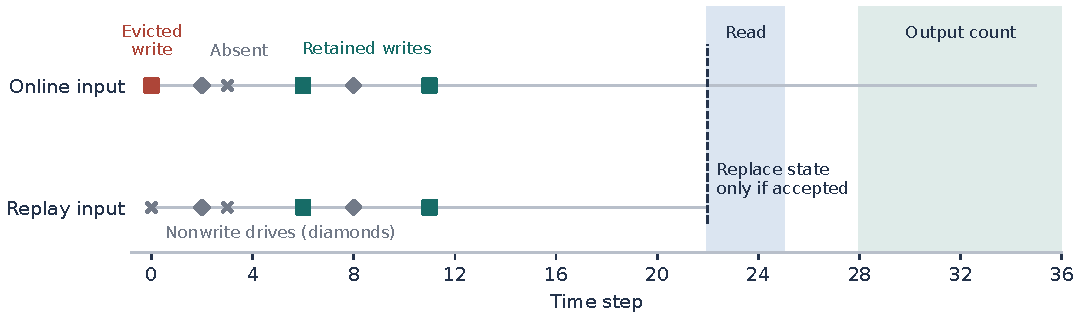
\includegraphics[width=0.96\linewidth]{figures/schedule-and-gate.pdf}
\caption{Schedule A and the replay decision. In the illustrated three-write history, write 1 has been evicted, write 2 is absent, and writes 3 and 4 remain in the FIFO. Replay omits evicted and absent writes, retains nonwrite drives, and replaces native state at the first read. A competing evicted key can veto that replacement.}
\label{fig:policy}
\end{figure}

\subsection{Evidence sequence and frozen tests}
The earlier learned-key study used 12 paired training blocks and three matching conditions. Subsequent fixed-weight interference, donor, reset, and replay studies reused trained models to isolate candidate mechanisms. These related explorations informed later freezes. We report them separately from the two confirmation cohorts.

\begin{table}[htbp]
\centering
\caption{Two fresh confirmation cohorts. A path is one geometry, history, and policy evaluated on all episodes in a block. A block, rather than a path or an episode, is the independent resampling unit.}
\label{tab:cohorts}
\small
\begin{tabularx}{\linewidth}{@{}lcccrX@{}}
\toprule
Cohort & New fits & Episodes/block & Geometries & Paths & Prespecified comparison \\
\midrule
Replay & 12 & 512 & 1 & 96 & Old replay vs. original on orthogonal three-write histories \\
Veto & 12 & 256 & 2 & 288 & Veto vs. old replay on near-neighbor three-write histories \\
\bottomrule
\end{tabularx}
\end{table}

For each cohort, twelve newly trained parameter vectors and update ledgers were locked before held-out generation. Every block uses matched episodes across its paths, including the four fixed schedules in Table~\ref{tab:schedules}. The original replay study tests improvement on recent records and noninferiority on evicted records. The veto study tests improvement on evicted records and noninferiority on recent records. For each endpoint, within a block we average the two three-write history differences equally. We resample the twelve paired blocks together 50,000 times and report the 1.25th and 98.75th percentiles \cite{efron1979}. The lower bound must exceed zero for improvement and $-2\pp$ for noninferiority. Both endpoints must pass. The two 97.5\% intervals follow each study's frozen nominal multiplicity convention. Their percentile coverage is approximate with twelve blocks. Other subgroups and engineering measures are descriptive. The veto bootstrap seed is \texttt{4087900001}.

\section{Results}
\subsection{Routing and native state are separable in this task}
The learned-key study found a LEARN-minus-MEAN difference of $52.28\pp$ on opposite-content balanced accuracy, with a 97.5\% interval $[42.71,62.37]$. An opposite-class read swap gave a $96.48\pp$ paired answer effect in the specified assay. These interventions establish that the read pathway participates in the native answer in those fitted circuits. In a subsequent interference study using the same trained family, native-state replacement raised recent BA by $10.30\pp$ $[8.61,12.00]$. Value replacement raised it by $0.67\pp$ $[0.13,1.22]$. In a donor-content control, matching-content donors produced a 5.769-spike advantage in label-aligned count difference over donors with a flipped target bit $[5.089,6.435]$. This effect survived fixed read injection. These differences identify component effects in the imposed substitutions and are not additive decompositions of natural computation.

Several alternative interventions had limited support. In the tested learned family, selective zeroing and a fixed warm state each failed to establish the prespecified recent-record benefit. In the broader programme, a pilot of the original TAN population produced zero native counts, and a fresh dual-scale attention cohort failed its common superiority hypothesis. These outcomes are included in the release lineage. They delimit the architecture and training conditions from which the final replay policy was developed.

\subsection{Old replay improves recent reads on new fits}
In the independent replay cohort, old replay improved recent-record BA by $5.273\pp$ with interval $[3.418,7.161]$, compared with the original circuit. The evicted-target difference was $-0.130\pp$ $[-0.521,0.000]$. Both lower bounds exceeded their prespecified thresholds. This cohort used orthogonal keys and a different held-out sample size. Its estimates remain separate from the veto cohort.

\subsection{Evicted-key competition selectively removes harmful replay}
In the fresh veto cohort, the near-neighbor three-write evicted-target difference was $+0.781\pp$ $[+0.130,+1.563]$. Four blocks improved and eight had zero change. The four positive differences were $3.125$, $3.125$, $1.563$, and $1.563\pp$. The recent-record difference was zero in every block and its interval collapsed to $[0,0]$. Both frozen endpoints passed (Figure~\ref{fig:effects}).

\begin{table}[htbp]
\centering
\caption{Mean block BA in the primary near-neighbor three-write histories, and the paired veto effect. Values use all examples in their target class, including episodes that do not trigger and tied outputs. The interval is in percentage points.}
\label{tab:veto}
\small
\begin{tabular}{@{}lrrrrl@{}}
\toprule
Target & Original & Old replay & Veto & Veto $-$ replay & 97.5\% interval \\
\midrule
Evicted & 59.115\% & 58.333\% & 59.115\% & $+0.781$ & $[+0.130,+1.563]$ \\
Recent & 89.909\% & 96.094\% & 96.094\% & $0.000$ & $[0.000,0.000]$ \\
\bottomrule
\end{tabular}
\end{table}

\begin{figure}[htbp]
\centering
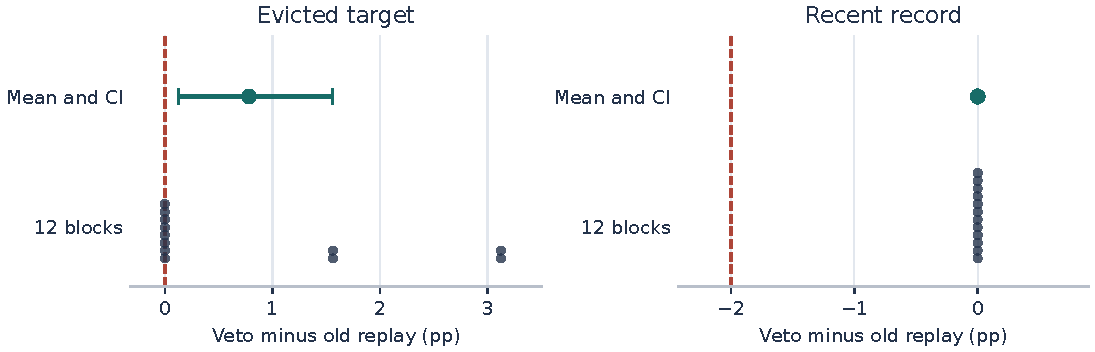
\includegraphics[width=0.98\linewidth]{figures/primary-effects.pdf}
\caption{Primary paired veto effects in the 12 fresh training blocks. The point and bar show the mean and 97.5\% paired-block interval. The vertical dashed line marks the endpoint-specific decision threshold. Points below the estimate are block differences. The recent endpoint has twelve zero differences.}
\label{fig:effects}
\end{figure}

The veto canceled 368 old triggers on evicted targets across the two near-neighbor three-write histories. These changes yielded 12 additional correct answers and removed none. Evicted-target BA returned to the original model's level (Table~\ref{tab:veto}). The mechanism therefore corrects an added loss from replay. The value of a discarded record is not put back into memory. Recent examples had no canceled triggers and kept the old replay benefit of $6.185\pp$ over the original model in the same cohort. The collapsed recent interval describes the twelve observed blocks. It does not guarantee equality for future fits.

In the descriptive near-neighbor four-write history, the veto canceled 368 evicted-target triggers and added 25 correct answers with no losses. In near three-write histories, 368 old triggers on missing targets remained. Those histories preserve the input equality of opposite-label missing-target pairs. Orthogonal histories retained all 4,608 old triggers. No policy reconstructed state in two-write histories. These controls locate the observed effect in competition between retained and evicted keys in the tested near geometries.

\subsection{Resources and timing}
Across the final paired evaluation, the veto removed 16,512 replay sample steps, corresponding to 2,575,872 native matrix multiply--accumulates within replay. It made 13,760 evicted-key comparisons and allocated a 32-byte evicted-key array per episode. Online resources changed separately. For example, near-neighbor recurrent deliveries increased from 12,226,848 under old replay to 12,228,732 under the veto. The engineering executor shares common trajectories and therefore has a separate cost ledger from the three logical model paths.

We timed 384 pairs of complete, independent from-zero calls, chosen from the first old triggers per schedule and geometry in the four-write history. The median paired latency change (veto minus replay) was $-0.150$ ms for the near geometry and $+0.481$ ms for the orthogonal geometry. Among 25 near pairs whose replay was canceled, it was $-3.168$ ms. These observations apply to the selected sample and this CPU implementation. Earlier cache and zero-row experiments removed 44.15\% of replay MACs but added 4.738 ms in batch and 0.961 ms in single calls in their fixture. Operation counts, memory, events, and latency are reported separately. No physical energy measurements were made.

\section{Reproducibility and limitations}
The frozen training records preserve seeds, initial and final parameters, native counts, and recorded gradients. For the final cohort, independent code reconstructed all 7,200 Adam updates, checked 36 native training forwards at endpoints, and independently replayed all 288 held-out paths. The audit recorded 129,404 checks and a maximum continuous residual of $4.44\times10^{-15}$. Discrete archived outputs matched exactly. These checks establish consistency with an independent implementation in the same research workflow. They do not constitute an external replication or an independent recomputation of every gradient.

The tasks use synthetic short sequences, two retained slots, a fixed FIFO rule, a fixed threshold, one trained population scaffold, and the tested key geometries and noise. Counterfactual replay estimates the effect of a specifically constructed prefix. It does not infer what an arbitrary trained recurrent state represents. Twelve independent blocks give limited resolution for rare errors and tails. The observed $0.781\pp$ increment is concentrated in four blocks and restores the original evicted-target level. Broader angle and noise sweeps, different memory capacities, and other implementations are open questions. The public evidence index retains null, failed, and budget-stopped phases and distinguishes them from completed scientific tests.

\section{Conclusion}
The experiments separate address selection from the native state that receives the read. Visible-event replay improved recent reads on fresh fits. An evicted-key veto repaired a small, localized loss introduced by that replay and preserved its benefit for recent records on the tested near-neighbor task. This is a reproducible example of a selective correction to a learned recurrent solution. A useful next experiment is to test a prefix checkpoint with the same causal replay semantics and account for the online cost of maintaining it before comparing full-call latency.

\paragraph{Code and data availability.}
The \href{\repo/tree/main/research/dend-tan-2026-11}{research release} contains the frozen evidence lineage, portable code, synthetic counts and trigger records, primary statistics, and raw archive provenance. The \href{\repo/tree/main/papers/dend-tan-event-replay-2026}{paper directory} includes the editable source, figures, and build instructions. No human-subject or external training data were used in the reported confirmations.

\paragraph{Research assistance.}
Protocol formalization, implementation, execution, numerical checks, and manuscript preparation included AI assistance. The evidence files specify the scope of the independent implementation checks.

\begin{thebibliography}{9}
\bibitem{miller2016} A. Miller, A. Fisch, J. Dodge, A.-H. Karimi, A. Bordes, and J. Weston. Key-Value Memory Networks for Directly Reading Documents. \emph{EMNLP}, pp. 1400--1409, 2016. \href{https://doi.org/10.18653/v1/D16-1147}{doi:10.18653/v1/D16-1147}.
\bibitem{vaswani2017} A. Vaswani et al. Attention Is All You Need. \emph{Advances in Neural Information Processing Systems}, 30, 2017. \href{https://proceedings.neurips.cc/paper/2017/hash/3f5ee243547dee91fbd053c1c4a845aa-Abstract.html}{Proceedings record}.
\bibitem{tanrepo} Z. Li. \emph{Temporal Attention Neuron: Research programme and source archive}. 2026. \href{\repo}{Versioned repository}.
\bibitem{populations} Z. Li. \emph{Training Interactions, Recurrence Dependence, and Size Tradeoffs in Native-Spike Dendritic and Point Networks}. Unreviewed research manuscript, 2026. \href{\repo/tree/7dcddee41490d8d917936891989eeb7ddb67e0da/papers/native-spike-populations-2026}{Pinned source and evidence}.
\bibitem{zenke2018} F. Zenke and S. Ganguli. SuperSpike: Supervised Learning in Multilayer Spiking Neural Networks. \emph{Neural Computation}, 30(6):1514--1541, 2018. \href{https://doi.org/10.1162/neco_a_01086}{doi:10.1162/neco\_a\_01086}.
\bibitem{efron1979} B. Efron. Bootstrap Methods: Another Look at the Jackknife. \emph{Annals of Statistics}, 7(1):1--26, 1979. \href{https://doi.org/10.1214/aos/1176344552}{doi:10.1214/aos/1176344552}.
\end{thebibliography}
\end{document}
